\beginsong{In das Dorf}[
    wuw={aus dem Russischen}, 
    bo={202}, 
    pfii={35}, 
    pfiii={16}, 
    gruen={56}, 
    kssiv={28}, 
    siru={129},
]

\beginverse
\endverse
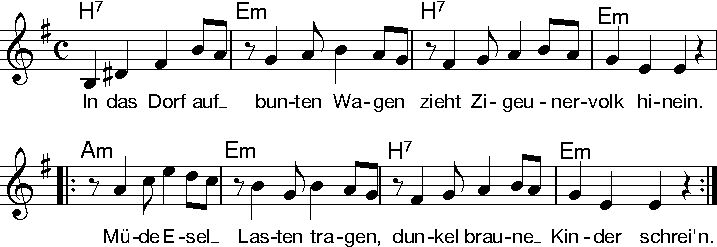
\includegraphics[draft=false, width=1\textwidth]{Noten/Lied053.pdf}	

\beginverse
\[H7]Bauern, in den \[Em]Stall die Schweine, \[H7]dem Zigeuner traue nie. \[Em]
\lrep \[Am]Nehmt die Wäsche \[Em]von der Leine, \[H7]rettet euer \[Em]Federvieh! \rrep
\endverse

\beginverse
^Kesselflicker, ^Scherenschleifer ^preisen ihre Künste laut. ^
\lrep ^Geiger spielen ^Korobuschka, ^schon tanzt Sven mit ^seiner Braut.\rrep
\endverse

\beginverse
^Mädchen, die auf ^Heirat warten, ^drängen sich an Maras Stand, ^
\lrep ^denn die Alte ^legt die Karten, ^liest die Zukunft ^aus der Hand.\rrep
\endverse

\beginverse
^Dudelsack quält ^ohne Pause, ^brauner Bär tanzt mit Gebrumm. ^
\lrep ^Spät geht frohes ^Volk nach Hause, ^dunkel liegt das ^Dorf und stumm.\rrep
\endverse

\endsong

\beginscripture{}
Die Melodie stammt vom russischen Motiv ''Korobeiniki''. Dieses ist in der westlichen Welt vor allem durch die ''Type A''-Musik aus Tetris für den Gameboy bekannt.
\endscripture
